\documentclass{article}
\usepackage[margin=.75in]{geometry}
\usepackage{libertine}
\usepackage[libertine]{newtxmath}
%\renewcommand{\ttdefault}{txtt}
\usepackage{DejaVuSansMono}
\usepackage[fontsize=10pt]{scrextend} % match document font size to label font used int Style program
\usepackage[inkscapearea=page]{svg} % import SVGs with same document size as specified in SVG
\usepackage[outline]{contour}
\contourlength{.1em}
\usepackage{mdframed}
\usepackage{xcolor}

% figure captions and labels
\usepackage[format=plain,
            labelfont={bf},
            textfont=sf]{caption}
\newcommand{\figlabel}[1]{\textsf{#1}}
\newcommand{\figloc}[1]{\textit{#1}}

\renewcommand{\labelitemi}{$\bullet$}
\renewcommand{\labelitemii}{---}
\renewcommand{\labelitemiii}{---}
\renewcommand{\labelitemiv}{---}

\usepackage{natbib}
\usepackage{xcolor}

\usepackage{minted}
\usemintedstyle{manni}
\definecolor{bg}{rgb}{0.95,0.95,0.95}
\newcommand{\code}[1]{\texttt{\small{#1}}}


\usepackage{soul}
\sethlcolor{yellow}
\newcommand{\todo}[1]{\textbf{\hl{TODO: #1}}}

\newcommand{\Eg}{\emph{E.g.}} % "for example"
\newcommand{\eg}{\emph{e.g.}} % "for example"
\newcommand{\Ie}{\emph{I.e.}} % "that is"
\newcommand{\ie}{\emph{i.e.}} % "that is"
\newcommand{\cf}{\emph{cf.\ }} % "confer"
\newcommand{\Etc}{\emph{Etc.}} % "et cetera" (and so on)
\newcommand{\etc}{\emph{etc.}} % "et cetera" (and so on)
\newcommand{\etal}{\emph{et al.}} % "and others"
\newcommand{\resp}{\emph{resp.}} % "respectively"
\newcommand{\ala}{\emph{\`{a} la}} % "in the style of"
\newcommand{\apriori}{\emph{a priori}} % based on deduction rather than experience
\newcommand{\aposteriori}{\emph{a posteriori}} % based on observation
\newcommand{\Aposteriori}{\emph{A posteriori}} % based on observation
\newcommand{\invivo}{\emph{in vivo}} % taking place in a living organism
\newcommand{\invitro}{\emph{in vitro}} % taking place in an artifical environment
\newcommand{\inutero}{\emph{in utero}} % taking place before birth
\newcommand{\adlibitum}{\emph{ad libitum}} % without preparation
\newcommand{\abinitio}{\emph{ab initio}} % without preparation


\newcommand{\St}{\text{St}}

% \renewcommand{\vec}[1]{\textbf{#1}}
\renewcommand{\vec}[1]{#1}


\title{\textsc{Walk on Stars} \\ \Large{(Implementation Guide)}}
\author{Rohan Sawhney, Bailey Miller, Ioannis Gkioulekas, Keenan Crane}
\date{}

\begin{document}

\maketitle

\begin{figure}[h!]
   \centering
   \begin{minipage}{150pt}
      \centering
      \figlabel{\phantom{mmmm}\textsc{Walk on Spheres}} \\
      \includesvg{images/WalkOnSpheres.svg}
   \end{minipage}
   \begin{minipage}{250pt}
      \centering
      \figlabel{\textsc{Walk on Stars}\phantom{mmmmm}} \\
      \includesvg{images/WalkOnStars.svg}
   \end{minipage}
   \caption{Walks taken by the WoS algorithm \emph{(left)} and the WoSt algorithm \emph{(right)}.  The algorithms are virtually identical, except that WoSt replaces spheres with star-shaped regions, enabling walks to reflect off Neumann boundaries.\label{fig:WoSvsWoSt}}
\end{figure}

% \begin{figure}[h!]
%    \todo{Figure showing a polygonal domain $\Omega$, with the two boundary components drawn in different styles}
%    \caption{The domain for our problem.\label{fig:ProblemDomain}}
% \end{figure}

This note provides a step-by-step tutorial on how to implement the \emph{walk on stars (WoSt)} algorithm of \citet{Sawhney:2023:WoSt}.  Though the derivation of algorithm takes some work, the final algorithm remains about as simple as the original \emph{walk on spheres (WoS)} method of \citet{muller1956some}.  For a Laplace equation with Dirichlet boundary conditions, WoS essentially says:

\begin{mdframed}[backgroundcolor=black!10,rightline=false,leftline=false]
   \textsc{(Walk on Spheres)} \emph{Repeatedly jump to a random point on a \textbf{sphere} around the current point until you reach the boundary.  The average boundary value over many such walks yields the solution.}
\end{mdframed}

For a Laplace equation with Dirichlet and zero-Neumann boundary conditions, WoSt is nearly identical:

\begin{mdframed}[backgroundcolor=black!10,rightline=false,leftline=false]
   \textsc{(Walk on Stars)} \emph{Repeatedly jump to a random point on a \textbf{star-shaped region} around the current point until you reach the \textbf{Dirichlet} boundary.  The average boundary value over many such walks yields the solution.}
\end{mdframed}

The main implementation effort is in enriching the closest point queries used by WoS with \emph{closest silhouette point queries}, as well as standard ``first hit'' ray intersection queries.  A complete 2D implementation with no external dependencies is provided in about 150 lines of C++ code (ignoring I/O), in the file \code{WoStLaplace.cpp}.  For simplicity, we omit nonzero Neumann conditions and acceleration of geometric queries---full 3D implementation is detailed in \citet{Sawhney:2023:WoSt}.

To emphasize the core ideas of the WoSt algorithm, this tutorial focuses on a bare-bones 2D version of WoSt that solves the Laplace equation
\begin{equation}
   \label{eq:MainPDE}
   \begin{array}{rcll}
      \Delta u &=& 0 & \text{on}\ \Omega, \\
             u &=& g & \text{on}\ \partial\Omega_D, \\
             \tfrac{\partial u}{\partial n} &=& 0 & \text{on}\ \partial\Omega_N, \\
   \end{array}
\end{equation}
where \(\Omega \subset \mathbb{R}^2\) is a closed polygon in the plane, \(g\) is a real-valued function on the Dirichlet part of the boundary \(\partial\Omega_D\), and \(\partial\Omega_N\) is the complementary Neumann part of the boundary.  

\newpage

\section{Overview}
\label{sec:Overview}

\subsection{Walk on Spheres (WoS)}
\label{sec:WalkOnSpheresOverview}


A good way to understand WoSt is to start with the basic WoS algorithm, which solves the same problem but with pure Dirichlet boundary conditions (\(\partial_N = \O\)).  The basic idea is quite simple: to estimate the solution at a point \(\vec{x}_0 \in \Omega\), just take \(M\) random walks to the boundary \(\partial\Omega\) (for some large number \(M\)), and grab the average value \(g\) at these boundary points.  The average boundary value across all walks then gives an estimate of the solution, which becomes more accurate as \(M\) increases.  The reason this method is called ``walk on \emph{spheres}'' is that these random walks are simulated by repeatedly jumping to the boundary of the largest empty sphere \(S_r(\vec{x}_k) \subset \Omega\) around the current point \(\vec{x}_k\) to get the next point \(\vec{x}_{k+1}\).  Steps hence tend to be big, and the method quickly makes progress toward the boundary (in comparison to taking small, fixed-sized steps).  In a bit more detail, the WoS algorithm looks like this:

\begin{itemize}
   \item \textbf{for} \(i = 1, \ldots, M\):
\begin{itemize}
   \item \textbf{until} \(\vec{x}_k\) is within a small distance \(\varepsilon\) of the domain boundary \(\partial\Omega\):
      \begin{itemize}
         \item Compute the distance \(r\) to the closest point \(\overline{\vec{x}}_k\) on \(\partial\Omega\).
         \item Pick a random point \(\vec{x}_{k+1}\) on the sphere \(S_r(\vec{x}_k)\) of radius \(r\) around \(\vec{x}_k\).
      \end{itemize}
   \item Add the value of \(g(\overline{\vec{x}}_k)\) to a running total \(\widehat{u}\).
\end{itemize}
   \item Return the estimate \(\widehat{u}/M\).
\end{itemize}

Figure \ref{fig:WoSvsWoSt}, \figloc{left} shows an example walk.  To actually implement this algorithm, we just need two kinds of subroutines:
\begin{itemize}
   \item \textbf{Geometric queries.}  For a given point \(\vec{x}_k \in \Omega\), we need to know how to compute the closest point \(\overline{\vec{x}}_k\) on the boundary.
   \item \textbf{Random sampling.} For a sphere \(S\) with center \(\vec{x}_k\) and radius \(r\), we need to know how to pick a point \(\vec{x}_{k+1}\) on \(S\) uniformly at random.
\end{itemize}

In fact, this basic structure will be the same for any ``walk on X'' algorithm (known more broadly as \emph{grid-free Monte Carlo methods}).  We generally need to perform some small set of geometric queries, and sample from some small set of probability distributions.  Otherwise, the logic is pretty similar: repeatedly apply these operations to simulate a random walk, and average values obtained from each walk to get the final solution estimate.


\subsection{Walk on Stars (WoSt)}
\label{sec:WalkOnStarsOverview}

\begin{figure}[h!]
   \centering
   \includesvg{images/StarShapedRegion.svg}
   \includesvg{images/StarShapedRadii.svg}

   \caption{\figloc{Left:} a region \(R\) is \emph{star shaped} relative to a point \(\vec{x}\) if every point \(\vec{y} \in R\) is visible from \(\vec{x}\) along a straight line. \figloc{Right:} WoSt identifies star shaped regions \(\St\) by finding the largest ball that contains neither the Dirichlet boundary nor the silhouette of the Neumann boundary.\label{fig:StarShapedRegions}}
\end{figure}

The WoSt algorithm is almost like the WoS algorithm, except that it simulates random walks that ``reflect'' off the Neumann boundary \(\partial\Omega_N\), in addition to the walks already ``absorbed'' into the Dirichlet boundary \(\partial\Omega_D\).  To do so, WoSt makes just two small changes to WoS.  First, in place of spheres \(S(\vec{x})\), WoSt uses \emph{star-shaped regions} \(\St(\vec{x})\) (see Figure~\ref{fig:StarShapedRegions}).  Unlike the spheres used by WoS, which touch the boundary only at isolated points, the star-shaped regions used by WoSt can include large pieces of the Neumann boundary \(\partial\Omega_N\).  Second, rather than terminating walks at all boundaries, WoSt continues walking from any point on the Neumann part of the boundary \(\partial\Omega_N\).  The overall flow now goes like this:

\begin{itemize}
   \item \textbf{for} \(i = 1, \ldots, M\):
\begin{itemize}
   \item \textbf{until} \(\vec{x}_k\) is within a small distance \(\varepsilon\) of the Dirichlet boundary \(\partial\Omega_D\):
      \begin{itemize}
         \item Compute the distance \(d_{\text{Dirichlet}}\) to the closest point on \(\partial\Omega_D\).
         \item Compute the distance \(d_{\text{Silhouette}}\) to the closest \emph{silhouette point} on \(\partial\Omega_N\).
         \item Let \(r := \min(d_{\text{Dirichlet}},d_{\text{Silhouette}})\).
         \item Shoot a ray from \(\vec{x}_k\) in a random direction \(v\), letting the next point \(\vec{x}_{k+1}\) be the first point where the ray hits either (i) the sphere \(S(\vec{x}_k,r)\), or (ii) the Neumann boundary \(\partial\Omega_N\).
      \end{itemize}
   \item Add the value of \(g(\overline{\vec{x}}_k)\) to a running total \(\widehat{u}\).
\end{itemize}
   \item Return the estimate \(\widehat{u}/M\).
\end{itemize}

Here we've omitted a couple small but important details which we'll cover later---\eg{}, the ray \(\vec{v}\) must be sampled from a hemisphere rather than a sphere if \(\vec{x}_k\) is on the boundary, and we generally want to set some minimum radius \(r_{\min}\).  But our final implementation really won't be much more complicated than the short outline above.  The main thing you may notice is that we now have three geometric queries to implement: a \emph{closest point query}, a \emph{closest silhouette point query}, and a \emph{closest ray intersection}.  We'll first walk through how to implement these queries in Section~\ref{sec:GeometricQueries}, followed by a more detailed implementation of WoSt in Section~\ref{sec:WalkOnStars}.

\begin{figure}[h!]
   \centering
   \begin{minipage}{150pt}
      \centering
      \includesvg{images/WalkOnStarsTrajectories.svg} \\
      \figlabel{(test problem)}
   \end{minipage}
   \begin{minipage}{150pt}
      \centering
      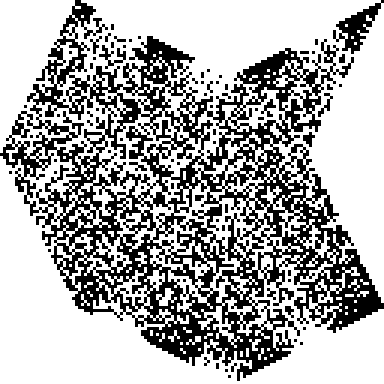
\includegraphics[width=150pt]{images/WoSt-1wpp.png} \\
      \figlabel{1 walk/point}
   \end{minipage}
   \begin{minipage}{150pt}
      \centering
      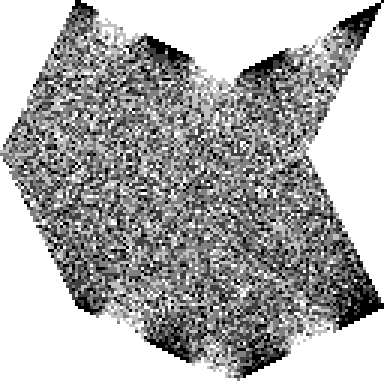
\includegraphics[width=150pt]{images/WoSt-4wpp.png} \\
      \figlabel{4 walks/point}
   \end{minipage}

   \vspace{\baselineskip}

   \begin{minipage}{150pt}
      \centering
      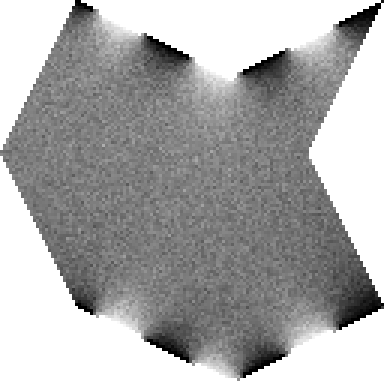
\includegraphics[width=150pt]{images/WoSt-128wpp.png} \\
      \figlabel{128 walks/point}
   \end{minipage}
   \begin{minipage}{150pt}
      \centering
      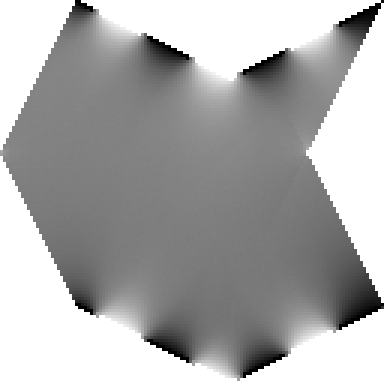
\includegraphics[width=150pt]{images/WoSt-65536wpp.png} \\
      \figlabel{reference}
   \end{minipage}
   \caption{Example walks taken by the WoSt algorithm are shown at \figloc{top, left}.  Taking more and more walks per point (blue lines), and averaging the resulting boundary values (white points), yields a smoother and more accurate solution estimate \figloc{(bottom right)}.\label{fig:WoSExample}}
\end{figure}

\newpage

\section{Geometric Queries}
\label{sec:GeometricQueries}

Numerous algorithms in visual, geometric, and scientific computing must perform \emph{geometric queries}: given a piece of geometry (\eg{}, a polygon mesh or implicit surface), answer some question about this geometry, relative to a query point \(x\) (\eg{}, how far away is the closest point?).  Many queries are well-studied, with extremely efficient implementations available on a variety of platforms.  When the number of geometric primitives gets very large (\eg{}, thousands or millions of triangles), it becomes especially important to use a \emph{spatial data structure} like a bounding volume hierarchy (BVH) or binary space partition (BSP) to accelerate computation.  To keep things simple, we'll here just assume that the number of primitives is small, and check each primitive directly.  For an implementation-oriented introduction to spatial data structures, see \citet[Section 4.2]{pharr2016physically}.

\paragraph{Assumptions.} To keep our discussion (and our code) simple, we'll assume that the geometry of the domain \(\Omega\) is a collection of closed simple polygons in the 2D plane, possibly with holes.  More explicitly, we'll assume we're given two lists of polylines: one for the Dirichlet boundary, and one for the Neumann boundary.  Each polyline is given by a list of 2D points \(\vec{p}_0, \ldots, \vec{p}_m \in \mathbb{R}^2\), which are encoded via a \code{Vec2D} type with all the usual 2D vector operations.  We also assume that all polylines have a consistent winding direction---for instance, if the domain is the letter ``A'', then polylines around the outer boundary should go in counter-clockwise order, and polylines around the inner hole should go in clockwise order (see Figure~\ref{fig:InsideOutside}).  This final assumption will just make it easier to get a consistent normal direction, and to do inside-outside tests if needed.  In fact, most of these assumptions are not strictly required by the WoSt algorithm itself; they largely just make coding easier.  See especially \citet[Appendix B]{Sawhney:2023:WoSt} for handling of ``messier'' input geometry.

\mbox{}

Here we break each query down into an ``atomic'' query for a single line segment, and a ``global'' query which basically just applies the atomic query to each segment in the overall list of polylines.

\subsection{Closest Point Query}
\label{sec:ClosestPointQuery}

A \emph{closest point query} seeks the point closest to the geometry relative to a given query point \(\vec{x}\).  Although closest point queries sometimes come up in the context of signed distance fields, we won't need to worry about sign or orientation here: we simply want to find the closest point, full stop.

\begin{figure}[h!]
   \centering
   \includesvg{images/AtomicClosestPoint.svg}
   \includesvg{images/ClosestPoint.svg}
   \caption{\figloc{Left:} given a query point \(\vec{x}\), the closest point \(\vec{y}\) on a line segment between \(\vec{a}\) and \(\vec{b}\) can be at either an interior point (\(0 < t < 1\)) or one of the endpoints (\(t=0,1\)). \figloc{Right:} The closest point on the boundary of our polygonal domain is then just the closest point among all segments in the domain boundary (here each black point is connected to the closest white point).\label{fig:ClosestPointExamples}}
\end{figure}

\paragraph{Atomic.} Given a query point \(\vec{x}\), we want to find the closest point on a line segment with endpoints \(\vec{a}, \vec{b}\) (Figure~\ref{fig:ClosestPointExamples}).  To find this point, we could first find the closest point on the full line, check if it's inside the segment, and if not, take the closer of the two endpoints.  Fortunately, all these operations boil down to a very simple subroutine (\citet{Quilez:2020:SLS} gives a nice derivation):

\inputminted[fontsize=\small,linenos,firstline=36,lastline=41,bgcolor=bg]{cpp}{../code/WoStLaplace2D.cpp}

\paragraph{Global.} To find the distance from a query point \(x\) to a collection of polylines, we now just need to apply our atomic closest point query to all segments and keep the smallest distance:

\inputminted[fontsize=\small,linenos,firstline=65,lastline=75,bgcolor=bg]{cpp}{../code/WoStLaplace2D.cpp}
The function \(\code{length}\) computes the length of the given vector, and the constant \code{infinity} is equal to floating-point infinity (\code{Inf}); as long as the polylines \code{P} contain at least one segment, the final distance \code{d} will be a finite value.

\subsection{Closest Silhouette Point Query}
\label{sec:ClosestSilhouettePointQuery}

\begin{figure}[h!]
   \centering
   \includesvg{images/AtomicClosestSilhouetteExample1.svg} \(\qquad\)
   \includesvg{images/AtomicClosestSilhouetteExample3.svg} \(\qquad\)
   \includesvg{images/AtomicClosestSilhouetteExample2.svg}
   \caption{A point \(\vec{b}\) is a \emph{silhouette point} if the segments \(\vec{a}\vec{b}\) and \(\vec{b}\vec{c}\) are front- and back-facing relative to a point \(\vec{x}\), or vice-versa.}
\end{figure}

Silhouette points are points where geometry changes from front-facing to back-facing, relative to a query point \(\vec{x}\).  A \emph{closest silhouette point query} seeks the closest such point along the entire silhouette.  In general, queries of the visibility silhouette are far less common than closest ray or closest point queries---a good reference is the work on \emph{spatialized normal cone hierarchies (SNCH)} by \citet{johnson2001spatialized}; \citet[Section 5.1]{Sawhney:2023:WoSt} explains how to accelerate closest silhouette point queries using an SNCH.  Here we'll again just perform brute-force evaluation, rather than use an acceleration scheme.

\paragraph{Atomic.} Given a query point \(\vec{x}\), we want to determine whether the point \(\vec{b}\) on a connected pair of line segments \(\vec{a}\vec{b}\), \(\vec{b}\vec{c}\) is a silhouette point.  Equivalently, we want to know if \(\vec{x}\) is on opposite sides of these two segments (\eg{}, in front of \(\vec{a}\vec{b}\) and behind \(\vec{b}\vec{c}\)).  We can easily check which side of \(\vec{a}\vec{b}\) the point \(\vec{x}\) is on by just computing the determinant of the vectors \(\vec{u} := \vec{a}-\vec{x}\) and \(\vec{v} := \vec{b}-\vec{x}\), which is equivalent to the signed area of triangle \(xab\).  Explicitly, \(\det(\vec{u},\vec{v}) = \vec{u}_1 \vec{v}_2 - \vec{u}_2 \vec{v}_1\).  Since this operation looks a lot like a cross product, we'll call it \code{cross} rather than \code{det} in our code (which also helps to distinguish it from \code{dot}!).  Our final routine is the quite simple:

\inputminted[fontsize=\small,linenos,firstline=43,lastline=46,bgcolor=bg]{cpp}{../code/WoStLaplace2D.cpp}

The logic here is simply that if \(\vec{x}\) is on the same side of both segments, then the determinants will have the same sign---hence their product will be positive.  Otherwise it will be negative.

\paragraph{Global.} To find the distance to the closest silhouette point we can once again iterate over all the geometry, check if each point is a silhouette point, and keep track of the closest distance seen so far:

\inputminted[fontsize=\small,linenos,firstline=77,lastline=88,bgcolor=bg]{cpp}{../code/WoStLaplace2D.cpp}
Note that in this code we check only the interior vertices of the polyline (by skipping the first and last index), since we assume that the domain boundary includes no open curves.  In general, however, one should account for the possibility that the endpoints of a polyline may be silhouette points.  Closed pure-Neumann loops can still be represented in the present code, by just repeating the points \(\vec{p}_0, \vec{p}_1\) at the end of the list.

Note that if all evaluation points \(x_0\) are inside the domain, an easy acceleration is to pre-process the Neumann boundary and keep only concave edge pairs (or triangle pairs, in the 3D case).  We do not however implement that acceleration here.

\subsection{Closest Ray Intersection}
\label{sec:ClosestRayIntersection}

\begin{figure}[h!]
   \centering
   \includesvg{images/AtomicClosestRay.svg}
   \includesvg{images/FirstRay.svg}
   \label{fig:RayIntersectionExample}
   \caption{\emph{Left:} a ray-segment intersection computes the time \(t \in (0,\infty)\) at which the ray \(r(t) = x + tv\) intersects the segment, and the parameter \(s \in [0,1]\) describing the location of the hit point along the line containing the segment. \emph{Right:} the first point where a ray hits a polygonal boundary then corresponds to the smallest positive \(t\) value.}
\end{figure}

Finally, given a point \(\vec{x}\) and a direction \(\vec{v}\), a \emph{closest ray intersection query} seeks the ``time'' \(t\) at which the ray \(\vec{x} + t\vec{v}\) first hits a given set.  In our case the set we want to consider is the boundary of the star-shaped domain \(\St(\vec{x},r)\).  Equivalently, we want to find the first \(t\) such that the ray hits either (i) the sphere \(S_r(\vec{x})\) of radius \(r\) around \(\vec{x}\), or (ii) the Neumann boundary \(\partial\Omega_N\) of the domain.  Our atomic query is still just an ordinary ray-segment intersection; logic in the global query then takes care of the ball radius.

\paragraph{Atomic.} There are many ways to derive (and implement) ray-segment intersection, but the basic idea is that if we express the line along the ray as \(\vec{f}(t) := \vec{x} + t\vec{v}\) and the line along the segment as \(\vec{g}(s) := (1-s)\vec{a} + s\vec{b}\), then we want to solve for the values \(s,t\) such that \(\vec{f}(t) = \vec{g}(s)\), \ie, the point at which the two lines coincide.  We then check whether \(s\) is between 0 and 1 (\ie, the intersection is within the segment) and \(t > 0\) (\ie, the intersection is in the direction of the ray).  After some algebraic manipulation, we arrive at one possible implementation:

\inputminted[fontsize=\small,linenos,firstline=48,lastline=60,bgcolor=bg]{cpp}{../code/WoStLaplace2D.cpp}

\paragraph{Global.} To find the first hit, we can now iterate over all segments in the given polylines and keep the minimum time \(t\) at which any intersection occurs.  Since we also want to intersect with a sphere of given radius \(r\), we can use \(r\) as the initial value for \(t\)---if we never encounter a closer segment, then we've hit the sphere:

\inputminted[fontsize=\small,linenos,firstline=90,lastline=113,bgcolor=bg]{cpp}{../code/WoStLaplace2D.cpp}

Notice that we compute the location \(x\) and normal \(n\) of the intersection point, as well as a flag \code{onBoundary} indicating whether the hit occurred on the domain boundary (rather than the sphere), which we'll need for the WoSt algorithm.  As is common practice in ray tracing, we also offset the ray origin by a small distance \(c\) so that the intersection point we find is not just the ray origin \(x\); a more numerically robust treatment of ray offsetting is described by \citet{wachter2019fast}.

\section{Walk on Stars}
\label{sec:WalkOnStars}

With all of our geometric queries in place, the actual WoSt algorithm is quite short.  The input is a query point \(\vec{x}_0\), a collection of polylines specifying the Dirichlet and Neumann parts of the boundary, and a function \(g\) that evaluates the Dirichlet value at any point \(x\) near the Dirichlet boundary \(\partial\Omega_D\):

\inputminted[fontsize=\small,linenos,firstline=119,lastline=126,bgcolor=bg]{cpp}{../code/WoStLaplace2D.cpp}

Here we also specify several solver parameters, which provide trade offs between speed and accuracy:
\begin{itemize}
   \item a value \(\varepsilon > 0\) which says how close we need to get to the Dirichlet boundary before we stop and grab the boundary value,
   \item the parameter \(r_{\min} > 0\) similarly limits how small our steps will shrink near the silhouette,
   \item the \code{nWalks} parameter says how many total walks we should take (hence how many boundary values we should average) to get our solution estimate, and
   \item the \code{maxSteps} parameter limits the number of steps taken by any walk.
\end{itemize}
The value \code{sum} will be used to accumulate all the values \(g\) we encounter at the boundary; normalizing this value by the number of walks gives us our final Monte Carlo estimate of the solution.  

At the beginning of each step, we assume that we're at an interior point (and hence the normal \(n\) is not well-defined):

\inputminted[fontsize=\small,linenos,firstline=128,lastline=132,bgcolor=bg]{cpp}{../code/WoStLaplace2D.cpp}

For each step, the first thing we do is compute the radius of the ball used to define a star shaped region \(\St(\vec{x},r)\).  This radius is the either the distance to the Dirichlet boundary, or the distance to the silhouette of the Neumann boundary---whichever one is closer.  We also limit the ball size to be at \emph{least} as big as the smallest step size parameter \(r_{\min}\):

\inputminted[fontsize=\small,linenos,firstline=134,lastline=141,bgcolor=bg]{cpp}{../code/WoStLaplace2D.cpp}

Next, we shoot a ray from the current point \(x\) in a random direction \(v\).  If \(x\) is on the domain interior, then we sample \(v\) from the full sphere (or in 2D: circle) around \(x\); if it's on the boundary, then we sample the hemisphere around the inward-pointing normal direction \(v\), so that the next point ends up inside the domain:

\inputminted[fontsize=\small,linenos,firstline=143,lastline=149,bgcolor=bg]{cpp}{../code/WoStLaplace2D.cpp}

Recall that the routine \code{intersectPolylines} will also update the flag \code{onBoundary}, and sets the normal \(n\) if the new point is on the boundary.  This loop continues taking steps along the walk until we get within a small distance \(\varepsilon\) of the Dirichlet boundary, or until we've exceeded the maximum number of steps---at this point we stop walking, and add the boundary contribution at the final location of \(\vec{x}\):

\inputminted[fontsize=\small,linenos,firstline=151,lastline=159,bgcolor=bg]{cpp}{../code/WoStLaplace2D.cpp}

After all walks are finished we return the average boundary value, which gives our solution estimate.  Figure~\ref{fig:WoSvsWoSt}, \figloc{right} shows an example walk.  (If you're curious about \emph{why} this algorithm works, you'll have to take a look at the full paper!)

\section{Inside-Outside Test (optional)}
\label{sec:InsideOutsideTest}

Though not strictly part of the WoSt algorithm itself, we may also want to know whether a given evaluation point \(\vec{x}_0\) is inside or outside the problem domain \(\Omega\) (\eg, for visualizing the solution).  To answer this query, we can just measure the total signed angle of the boundary polygon, relative to the query point:

\inputminted[fontsize=\small,linenos,firstline=191,lastline=202,bgcolor=bg]{cpp}{../code/WoStLaplace2D.cpp}

This signed angle is computed by just looping over all segments in the polylines, and adding up the signed angle of the individual segments.  If we represent points by complex numbers, the angle for a segment with endpoints \(\vec{a},\vec{b}\) is just \(\theta := \arg((\vec{b}-\vec{x})/(\vec{a}-\vec{x}))\), \ie, the angle that rotates the vector \(\vec{a}-\vec{x}\) to the vector \(\vec{b}-\vec{x}\):

\inputminted[fontsize=\small,linenos,firstline=182,lastline=189,bgcolor=bg]{cpp}{../code/WoStLaplace2D.cpp}

\begin{figure}[h!]
   \includesvg{images/AtomicSignedAngle.svg}
   \includesvg{images/SignedAngleInside.svg}
   \includesvg{images/SignedAngleOutside.svg}
   \caption{\emph{Left:} the signed angle subtended by segments \(ab\) and \(cd\) are positive and negative (\resp{}) with respect to \(x\). Summing these signed angles yields a total angle \(+2\pi\) for any point \(x\) inside a polygon \figloc{(center)}, and a total angle of zero for points \(x\) outside the polygon \figloc{(right)}.\label{fig:InsideOutside}}
\end{figure}


\section*{Acknowledgements} All diagrams in this document were made using \textsc{Penrose}~\citep{Ye:2020:PFM}.  Special thanks to Wode Ni, Sam Estep, Yiliang Liang, and the rest of the Penrose team for development support during production of this document.

\bibliographystyle{plainnat}
\bibliography{WoSt-tutorial}

\end{document}
